\section{Семантические модели и средства контроля знаний пользователей в ostis-системах}
\label{section_semantic_model_and_knowledge_control}

\begin{SCn}
	
	\begin{scnrelfromlist}{подраздел}
		\scnitem{\ref{subsec_research_results_problems_field_knowledge_control_automation}~\nameref{subsec_research_results_problems_field_knowledge_control_automation}}
		\scnitem{\ref{subsec_knowledge_control_automation}~\nameref{subsec_knowledge_control_automation}}
		\scnitem{\ref{subsec_semantic_model_KB_knowledge_control_subsystem}~\nameref{subsec_semantic_model_KB_knowledge_control_subsystem}}
		\scnitem{\ref{subsec_semantic_model_problem_solver_knowledge_control_subsystem}~\nameref{subsec_semantic_model_problem_solver_knowledge_control_subsystem}}
	\end{scnrelfromlist}
	
	\bigskip
	
	\begin{scnrelfromlist}{ключевое понятие}
		\scnitem{генерация тестовых вопросов}
		\scnitem{интеллектуальные обучающие системы}
		\scnitem{проверка ответов}
	\end{scnrelfromlist}
	
	\bigskip
	
	\begin{scnrelfromlist}{ключевое знание}
		\scnitem{установление отношений отображения онтологии}
		\scnitem{вычисление семантического сходства}
	\end{scnrelfromlist}
	
	\bigskip
	
	\begin{scnrelfromlist}{библиографическая ссылка}
		\scnitem{\scncite{Xu2009}}
		\scnitem{\scncite{Golenkov2001b}}
		\scnitem{\scncite{Golenkov2014b}}
		\scnitem{\scncite{Golenkov2019}}
		\scnitem{\scncite{Li2020}}
		\scnitem{\scncite{Li2021}}
		\scnitem{\scncite{IMS}}
		\scnitem{\scncite{Qian2020}}
		\scnitem{\scncite{Mousavinasab2018}}
		\scnitem{\scncite{SinghBhatia2013}}
		\scnitem{\scncite{Papasalouros2008}}		
		\scnitem{\scncite{Protege2016}}		
		\scnitem{\scncite{Li2012}}
		\scnitem{\scncite{Wan2019}}
		\scnitem{\scncite{Lix2009}}
		\scnitem{\scncite{Wan2019a}}
		\scnitem{\scncite{Shahmirzadi2019}}
		\scnitem{\scncite{Ji2022}}	
		\scnitem{\scncite{Anderson2016}}
		\scnitem{\scncite{Fujiwara2021}}
		\scnitem{\scncite{Zeng2021}}
		\scnitem{\scncite{Sun2020}}
		\scnitem{\scncite{Rujiang2011}}
		\scnitem{\scncite{Kowalski1974}}
		\scnitem{\scncite{Krom1970}}		
		\scnitem{\scncite{Zhang1995}}
		\scnitem{\scncite{Zhang2019}}		
		\scnitem{\scncite{Shunkevich2015}}
	\end{scnrelfromlist}
	
\end{SCn}

\section*{Введение в Параграф~\ref{section_semantic_model_and_knowledge_control}}
Данный параграф посвящен проблеме генерации тестовых вопросов и проверки ответов пользователей в \textit{интеллектуальных обучающих системах}. В данном параграфе подробно представлен подход к автоматической генерации тестовых вопросов различных типов на основе \textit{базы знаний} в \textit{интеллектуальных обучающих системах}, разработанных с использованием \textit{Технологии OSTIS}, и подход к реализации автоматической проверки ответов пользователей на основе различных семантических структур описанных знаний.

Применение технологии искусственного интеллекта в сфере образования может не только повысить эффективность обучения учащихся, но и стать важным средством обеспечения справедливости образования. Особенно после вспышки COVID-19 в 2020 году была подчеркнута важность и актуальность разработки \textit{интеллектуальных обучающих систем} (см. \scncite{Xu2009}). По сравнению с традиционной мультимедийной обучающей системой (м.о.с.), и.о.с. имеет следующие характеристики:

\begin{textitemize}
	\item способен вести свободный человеко-машинный диалог;
	\item предоставление персонализированной педагогической услуги;
	\item автоматическое решение тестовых вопросов;
	\item автоматическая генерация тестовых вопросов;
	\item автоматическая проверка ответов пользователей;
	\item и так далее.
\end{textitemize}

Среди перечисленных характеристик автоматическая генерация тестовых вопросов и автоматическая проверка ответов пользователей являются самыми основными и важными функциями и.о.с. Они позволяют автоматизировать весь процесс от генерации тестовых вопросов и формирования экзаменационных билетов до автоматической проверки ответов пользователей и оценки экзаменационных билетов. Это может не только значительно повысить эффективность тестирования уровня знаний пользователей, но и снизить стоимость их обучения, при этом исключая человеческий фактор, чтобы максимально обеспечить справедливость процесса тестирования.

Хотя в последние годы с развитием семантической сети, обработки естественного языка (NLP) и других соответствующих технологий некоторыми научно-исследовательскими группами были предложены и разработаны подходы и системы для автоматической генерации тестовых вопросов и автоматической проверки ответов пользователей, эти подходы и системы имеют много недостатков, таких как:

\begin{textitemize}
	\item только генерация простых объективных вопросов;
	\item большинство существующих подходов и систем проверки ответов поддерживает только проверку ответов пользователей на объективные вопросы;
	\item некоторые существующие подходы к проверке ответов пользователей на субъективные вопросы основаны на сопоставлении ключевых слов и статистике вероятности и не учитывают семантическое подобие между ответами;
	\item частично основанные на семантике подходы к проверке ответов пользователей на субъективные вопросы могут вычислять только подобие между ответами с простыми семантическими структурами;
	\item компоненты, разработанные с использованием существующих подходов к генерации тестовых вопросов и проверке ответов пользователей, могут быть использованы только в соответствующих системах;
	\item не поддерживается автоматизированная реализация всего процесса от генерации тестовых вопросов до проверки ответов пользователей (см. \scncite{Golenkov2014b}, \scncite{Golenkov2019}, \scncite{Li2020}).
\end{textitemize}

К типу вопросов с уникальным стандартным ответом относятся объективные вопросы, которые включают в себя: вопросы на выбор, вопросы суждения и вопросы на толкование определений. Субъективные вопросы не имеют уникальных ответов, а общие субъективные вопросы включают вопросы на доказательство, вопросы на толкование определений и решение задачи (см. \scncite{Li2021}).

В связи с этим в данном параграфе представлен подход к автоматической генерации тестовых вопросов и автоматической проверке ответов пользователей в обучающих системах, разработанных с использованием \textit{Технологии OSTIS}, и на основе предложенного подхода разработана универсальная подсистема для автоматической генерации тестовых вопросов и автоматической проверки ответов пользователей. Основной принцип автоматической генерации тестовых вопросов в данной работе заключается в том, чтобы сначала обобщить ряд стратегий генерации тестовых вопросов на основе структуры базы знаний ostis-систем и структуры представления знаний в ней, а затем использовать эти стратегии генерации тестовых вопросов для извлечения соответствующих семантических фрагментов из базы знаний и генерировать семантические модели, соответствующие тестовым вопросам (см. \scncite{Golenkov2014b}, \scncite{IMS}). Основной принцип проверки ответа на тестовый вопрос заключается в том, чтобы сначала вычислить подобие между семантическим фрагментом стандартного ответа и семантическим фрагментом ответа пользователя, а затем осуществить автоматическую проверку ответа пользователя на основе вычисленного подобия и стратегии оценки соответствующего тестового вопроса. Семантический фрагмент представляет собой сеть, которая отображает семантические отношения между понятиями. В ostis-системах семантический фрагмент строится с помощью \textit{SC-кода} (см. \scncite{IMS}, \scncite{Li2020}). Следует подчеркнуть, что семантический фрагмент, соответствующий тестовому вопросу, и соответствующее ему описание на естественном языке преобразуются друг в друга с помощью естественно-языковых интерфейсов (см. \scncite{Qian2020}). Подход, предложенный в данном параграфе, должен решить следующие задачи:

\begin{textitemize}
	\item автоматическая генерация ряда тестовых вопросов из базы знаний и сохранение их в соответствующих разделах базы знаний подсистемы;
	\item проектирование и построение баз знаний подсистем для хранения сгенерированных тестовых вопросов;
	\item извлечение соответствующих типов тестовых вопросов и составление экзаменационных билетов в соответствии с потребностями пользователей;
	\item вычисление подобия между семантическими фрагментами ответов на объективные вопросы;
	\item вычисление подобия между семантическими фрагментами ответов на вопросы на толкование определений;
	\item вычисление подобия между семантическими фрагментами ответов на вопросы на доказательство и на решение задачи;
	\item автоматическая проверка ответов на тестовые вопросы и автоматическая оценка экзаменационных билетов на основе вычисленного подобия и стратегии оценки соответствующих тестовых вопросов.
\end{textitemize}

Следует подчеркнуть, что предлагаемый в данном параграфе подход не опирается на какой-либо естественный язык, но для того, чтобы объяснить принцип работы предлагаемого подхода, подобранные в данном параграфе семантические фрагменты и иллюстрации представлены на русском языке. Среди них \textit{ostis-система} по дискретной математике и \textit{ostis-система} по евклидовой геометрии будут использоваться в качестве демонстрационных систем для подсистемы, разработанной с использованием предлагаемого подхода.

\subsection{Существующие научно-исследовательские результаты и проблемы в области автоматизации контроля знаний}
\label{subsec_research_results_problems_field_knowledge_control_automation}

\begin{SCn}
	\begin{scnrelfromlist}{подраздел}
		\scnitem{\ref{subsubsec_automatic_generation_test_questions}~\nameref{subsubsec_automatic_generation_test_questions}}
		\scnitem{\ref{subsubsec_automatic_checking_user_responses}~\nameref{subsubsec_automatic_checking_user_responses}}
	\end{scnrelfromlist}
\end{SCn}

\subsubsection{Автоматическая генерация тестовых вопросов}
\label{subsubsec_automatic_generation_test_questions}

Подход к автоматической генерации тестовых вопросов в основном изучает, как использовать электронные документы, корпуса текстов и базы знаний для быстрой и гибкой автоматической генерации тестовых вопросов. Благодаря тому, что знания в базе знаний представляют собой высокоструктурированные знания, прошедшие фильтрацию, и с развитием семантических сетей, использование базы знаний для автоматической генерации тестовых вопросов стало важнейшим направлением исследований в области автоматической генерации тестовых вопросов (см. \scncite{Xu2009, Mousavinasab2018, SinghBhatia2013}). Некоторые результаты исследований приведены ниже:

\begin{textitemize}
	\item подход к использованию классов, экземпляров, атрибутов и отношений между ними в онтологии OWL для генерации вопросов на выбор представлен в работе (см. \scncite{Papasalouros2008}). OWL представляет собой язык описания онтологий для семантической сети. Онтология – это вид знаний, каждое из которых является спецификацией соответствующей предметной области, ориентированной на описание свойств и взаимосвязей понятий, входящих в состав указанной предметной области; 
	\item подход к автоматической генерации объективных вопросов с использованием онтологии, созданной Protégé (см. \scncite{Protege2016}), представлен в работе (см. \scncite{Li2012}).
\end{textitemize}

Эти подходы в основном имеют следующие проблемы:

\begin{textitemize}
	\item подход к использованию электронных документов для автоматической генерации тестовых вопросов требует большого количества шаблонов предложений;
	\item создание корпуса текстов требует больших человеческих ресурсов для сбора и обработки различных знаний;
	\item существующие подходы могут быть использованы только в соответствующих системах и не являются совместимыми;
	\item существующие подходы позволяют генерировать только простые объективные вопросы.
\end{textitemize}

\subsubsection{Автоматическая проверка ответов пользователей}
\label{subsubsec_automatic_checking_user_responses}

Автоматическая проверка ответов пользователей делится на проверку ответов на объективные вопросы и проверку ответов на субъективные вопросы. Основной принцип проверки ответов на объективные вопросы относительно прост, то есть достаточно определить, совпадает ли строка стандартного ответа и строка ответа пользователя. Ответы на субъективные вопросы обычно не являются уникальными, поэтому основной принцип проверки ответов на субъективные вопросы заключается в вычислении подобия между стандартным ответом и ответом пользователя, а затем в осуществлении автоматической проверки ответов пользователя на основе вычисленного подобия и стратегии оценки соответствующих тестовых вопросов. Чем больше похожи стандартный ответ и ответ пользователя, тем выше подобие между ними (см. \scncite{Wan2019, Lix2009, Wan2019a}). Проверка ответов на субъективные вопросы делится на следующие категории в соответствии с подходом, используемым для вычисления подобия:

\begin{textitemize}
	\item На основе ключевых словосочетаний
	
	Этот тип подхода позволяет сначала разделить предложения на ключевые словосочетания, а затем вычислить подобие между ними в соответствии с отношениями совпадения ключевых словосочетаний между предложениями. Представительные подходы включают:
	
	\begin{textitemize}
		\item N-gram similarity
		\item Jaccard similarity
	\end{textitemize}
	
	\item На основе модели векторного пространства (VSM)
	
	Основной принцип VSM заключается в использовании традиционных алгоритмов машинного обучения для того, чтобы сначала преобразовать предложения в векторные представления, а затем вычислить подобие между ними (см. \scncite{Shahmirzadi2019}). Представительные подходы включают:
	
	\begin{textitemize}
		\item TF-IDF
		\item Word2vec
		\item Doc2Vec
	\end{textitemize}
	
	\item На основе глубокого обучения
	
	Этот тип подхода позволяет использовать модели нейронных сетей для вычисления подобия между предложениями (см. \scncite{Ji2022}). Представительные модели нейронных сетей включают:
	
	\begin{textitemize}
		\item Tree-LSTM
		\item Transformer
		\item BERT
	\end{textitemize}
	
	\item На основе семантического фрагмента
	
	Основной принцип вычисления подобия между ответами с использованием данного типа подхода заключается в том, чтобы сначала преобразовать ответы (то есть предложения или короткие тексты) в представление семантического фрагмента с помощью инструментов обработки естественного языка (например, синтаксические деревья зависимостей и естественно-языковые интерфейсы), а затем вычислить подобие между семантическими фрагментами (то есть подобие между ответами). В \textit{и.о.с.} различная информация хранится в виде семантических фрагментов, поэтому можно рассмотреть возможность вычисления подобия между любыми двумя семантическими фрагментами в базе знаний, опираясь на принципы работы данного типа подхода. Основным преимуществом этого типа подхода является вычисление подобия между ответами на основе семантики. Одним из наиболее представительных подходов является SPICE (Semantic Propositional Image Caption Evaluation) (см. \scncite{Anderson2016}). 
	
	Подход SPICE используется для вычисления подобия между автоматически сгенерированными подписями к рисункам (подписи-кандидаты) и подписями к рисункам, помеченными вручную (подписи-образцы). Данный подход позволяет вычислить подобие между подписями путем сопоставления одного и того же числа кортежей между семантическими кортежами подписи-кандидатов и семантическими кортежами подписи-образцов.
	
\end{textitemize}

Эти подходы в основном имеют следующие недостатки:

\begin{textitemize}
	\item подход, основанный на ключевых словосочетаниях, не учитывает порядок между словами в предложении;
	\item подход на основе VSM приводит к генерации высокоразмерных разреженных матриц, что увеличивает сложность алгоритма;
	\item подходы на основе семантических фрагментов, поддерживающие только описание простых семантических структур;
	\item эти подходы не позволяют определить, являются ли предложения логически эквивалентными друг другу;
	\item эти подходы зависят от соответствующего естественного языка.
\end{textitemize}

Поэтому на основе существующих подходов к автоматической генерации тестовых вопросов с использованием баз знаний, подходов к вычислению подобия между ответами с использованием семантических фрагментов и \textit{Технологии OSTIS} в данном параграфе предлагается подход к автоматической генерации тестовых вопросов и автоматической проверке ответов пользователей с использованием семантики.

\subsection{Предлагаемый подход к автоматизации контроля знаний}
\label{subsec_knowledge_control_automation}

\begin{SCn}
	\begin{scnrelfromlist}{подраздел}
		\scnitem{\ref{subsubsec_proposed_approach_automatic_generation_test_questions}~\nameref{subsubsec_proposed_approach_automatic_generation_test_questions}}
		\scnitem{\ref{subsubsec_suggested_approach_automated_checking_user_responses}~\nameref{subsubsec_suggested_approach_automated_checking_user_responses}}
		\scnitem{\ref{subsubsec_checking_answers_objective_questions}~\nameref{subsubsec_checking_answers_objective_questions}}
		\scnitem{\ref{subsubsec_checking_answers_subjective_questions}~\nameref{subsubsec_checking_answers_subjective_questions}}
	\end{scnrelfromlist}
\end{SCn}

Основной задачей данном параграфе является детализация подхода к автоматической генерации тестовых вопросов и автоматической проверке ответов пользователей в \textit{ostis-системах} и разработка универсальной подсистемы на основе этого подхода. Где универсальность подсистемы означает, что подсистема может быть легко перенесена между различными \textit{ostis-системами}. Предлагаемый подход можно разделить на две части в соответствии с реализуемыми функциями, то есть автоматическая генерация тестовых вопросов и автоматическая проверка ответов пользователей (см. \scncite{Li2021}). Поэтому мы представим процесс реализации этих двух частей отдельно.

\subsubsection{Предлагаемый подход к автоматической генерации тестовых вопросов}
\label{subsubsec_proposed_approach_automatic_generation_test_questions}

Основной принцип автоматической генерации различных типов тестовых вопросов (включая объективные вопросы и субъективные вопросы) в \textit{ostis-системах} заключается в том, чтобы сначала извлечь соответствующие семантические фрагменты из базы знаний, используя ряд стратегий генерации тестовых вопросов, обобщённых на основе подхода представления знаний и структуры описания знаний в рамках \textit{Технологии OSTIS}, затем добавить к извлечённым семантическим фрагментам информацию об описании тестового вопроса и, наконец, сохранить семантические фрагменты, описывающие полные тестовые вопросы, в соответствующем разделе подсистемы (см. \scncite{Golenkov2014b}). Когда необходимо сформировать экзаменационные билеты, подсистема позволяет извлечь из базы знаний подсистемы несколько соответствующих тестовых вопросов в соответствии с параметрами, введёнными пользователем, и объединить их в экзаменационные билеты. Тестовые вопросы и экзаменационные билеты в виде семантических фрагментов преобразуются в описания на естественном языке с помощью естественно-языковых интерфейсов. В работе (см. \scncite{Li2020}) мы подробно рассмотрели некоторые стратегии, используемые для автоматической генерации тестовых вопросов в \textit{ostis-системах}, далее мы выберем только некоторые из стратегий генерации тестовых вопросов для представления.

\begin{textitemize}
	\item Стратегия генерации тестовых вопросов на основе класса
	
	Этот тип стратегии генерации тестовых вопросов используется для автоматической генерации объективных вопросов, основанных на различных отношениях между классами. Далее она делится на:
	
	\begin{textitemize}
		\item На основе отношения \textit{включение*}
		
		Отношение включения является одним из наиболее часто используемых отношений в \textit{базе знаний ostis-систем}, которое удовлетворяется между многими классами (включая подклассы), поэтому отношение включения между классами может быть использовано для генерации объективных вопросов. Форма выражения в теории множеств отношения включения между классами выглядит следующим образом: $S_{i}\subseteq  C $, ($S$ – подкласс, $i$ – номер подкласса, $C$ – родительский класс). Ниже показан семантический фрагмент в базе знаний, который удовлетворяет отношению включения в \textit{SCn-коде} (см. \scncite{Golenkov2014b, IMS}): 
		\begin{SCn}
			\scnheader{бинарное дерево}
			\scnrelto{включение}{ориентированное дерево}
			\begin{scnrelfromlist}{включение} 
				\scnitem{братское дерево}
				\scnitem{дерево решений}
				\scnitem{бинарное дерево сортировки}
			\end{scnrelfromlist}
		\end{SCn}
		В качестве примера вопроса на выбор, сгенерированного с использованием этого семантического фрагмента на основе стратегии отношений включения, ниже показана его форма на естественном языке:
		
		<<Частным случаем бинарного дерева не является (\ )?>>
		
		A. дерево решений   \quad C. ориентированное дерево \\
		B. братское дерево  \quad D. бинарное дерево сортировки
		
		Пример семантической модели данного тестового вопроса приведён на рисунке (\textit{\nameref{fig:mc_example}}) в \textit{SCg-коде}.
		
		Аналогичным образом, используя эту стратегию, можно генерировать другие типы объективных вопросов;
		
		\item На основе отношения \textit{разбиение*}
		
		Отношение разбиения – это квазибинарное ориентированное отношение, областью определения которого является семейство всевозможных множеств. В  результате разбиения множества получается множество попарно непересекающихся множеств, объединение которых есть исходное множество. Отношение разбиения также является важным отношением в базе знаний, поэтому семантические фрагменты в базе знаний, удовлетворяющие этому отношению, могут быть использованы для генерации объективных вопросов. На языке теории множеств отношение разбиения между классами описывается следующим образом: $S_{i_{1}}\cup  S_{i_{2}}\cdots S_{i_{m}} \cup S_{i_{n}} = S_{j_{1}}\cup  S_{j_{2}}\cdots S_{j_{m}} \cup S_{j_{n}}= \cdots = U$, ($n>1$, $S_{j_{m}} \cap S_{j_{n}} = \oslash$). Ниже приведён семантический фрагмент в базе знаний, удовлетворяющий отношению \textit{разбиение*} в \textit{SCn-коде}:
		\begin{SCn}
			\scnheader{граф}
			\scnrelfrom{включение}{полуэйлеров граф}
			\begin{scnrelfromset}{разбиение}
				\scnitem{невзвешенный граф}
				\scnitem{взвешенный граф}
			\end{scnrelfromset}
			\begin{scnrelfromset}{разбиение}
				\scnitem{непланарный граф}
				\scnitem{планарный граф}
			\end{scnrelfromset}
			\begin{scnrelfromset}{разбиение}
				\scnitem{несвязный граф}
				\scnitem{связный граф}
			\end{scnrelfromset}
		\end{SCn}
		\begin{figure}[H]
			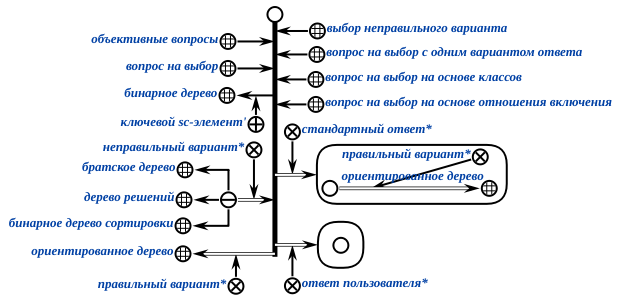
\includegraphics[scale=1]{author/part7/figures/MC_question_example.png}
			\caption{Пример семантической модели вопроса на выбор}
			\label{fig:mc_example}
		\end{figure}
		
		\item На основе отношения \textit{строгое включение*}
		
		Отношение строгого включения является особой формой отношения включения ($S_{i}\subset  C $, ($i\ge 1$)). Использование отношения строгого включения для автоматической генерации объективных вопросов аналогично использованию отношения включения. Ниже приведён семантический фрагмент в базе знаний, удовлетворяющий отношению \textit{строгое включение*} в \textit{SCn-коде}:
		
		\begin{SCn}
			\scnheader{Предметная область множеств}
			
			\begin{scnhaselementrolelist}{немаксимальный класс объектов исследования}
				\scnitem{счётное множество}
				\scnitem{ориентированное множество}
				\scnitem{конечное множество} 
				\begin{scnrelfromlist}{включение} 
					\scnitem{пара}
					\scnitem{тройка}
				\end{scnrelfromlist}
			\end{scnhaselementrolelist}
		\end{SCn}
	\end{textitemize}
	
\end{textitemize}	

Другие стратегии, используемые для генерации объективных вопросов, также включают:
\begin{textitemize}
	\item Стратегия генерации тестовых вопросов на основе элементов;
	\item Стратегия генерации тестовых вопросов на основе идентификаторов;
	\item Стратегия генерации тестовых вопросов на основе аксиом; 
	\item Стратегия генерации тестовых вопросов на основе атрибутов отношений;
	\item Стратегия генерации тестовых вопросов на основе примеров изображений.
\end{textitemize}

Конкретный процесс генерации объективных вопросов с использованием перечисленных выше стратегий подробно представлен в работе (см. \scncite{Li2020}).

Процесс генерации субъективных вопросов с использованием стратегии генерации субъективных вопросов выглядит следующим образом:

\begin{textitemize}
	\item поиск в базе знаний семантических фрагментов, описывающих субъективные вопросы с использованием логических правил (то есть шаблоны, построенные с использованием \textit{SC-кода});
	\item хранение найденных семантических фрагментов в соответствующем разделе базы знаний подсистемы;
	\item использование ручных подходов или автоматических подходов (например, с помощью естественно-языковых интерфейсов) для описания определения, процесса доказательства или процесса решения соответствующего тестового вопроса в соответствии с правилами представления знаний (то есть стандартные ответы на субъективные вопросы). Среди них стандартные ответы на субъективные вопросы представлены с помощью \textit{SCg-кода} или \textit{Языка SCL} (см. \scncite{Golenkov2014b, IMS}).
	
\end{textitemize}

Пример семантической модели субъективного вопроса показан на рисунке (\textit{\nameref{fig:DI_example}}) в \textit{SCg-коде}.

\begin{figure}[H]
	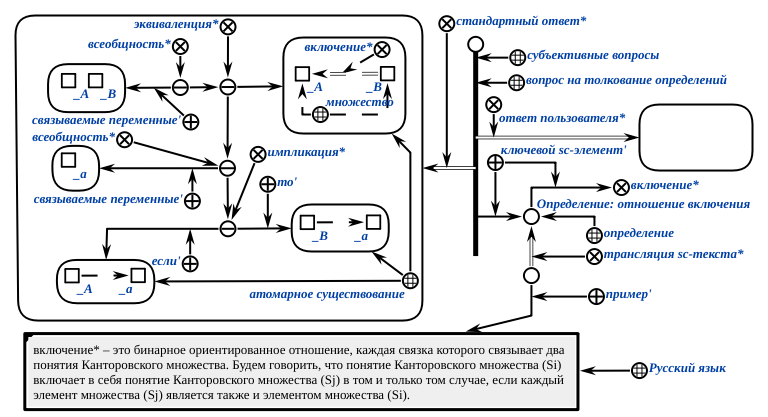
\includegraphics[scale=0.8]{author/part7/figures/DI_question_example.png}
	\caption{Семантическая модель определения отношения включения}
	\label{fig:DI_example}
\end{figure}

На рисунке (\textit{\nameref{fig:DI_example}}) описано определение отношения включения ($\forall A\forall B((A\subseteq B)\Longleftrightarrow (\forall a(a\in A\rightarrow a\in B))$).

Использование этих стратегий генерации тестовых вопросов, описанных выше, позволяет генерировать различные типы тестовых вопросов автоматически из базы знаний. Эти автоматически сгенерированные тестовые вопросы хранятся в базе знаний подсистемы в соответствии с их типом и соответствующей стратегией генерации тестовых вопросов. Такой тип хранения позволяет быстро и динамично генерировать экзаменационные билеты в соответствии с потребностями пользователя. В следующем подразделе мы подробно опишем построение базы знаний подсистемы и способ хранения в ней тестовых вопросов. Предлагаемый подход к генерации тестовых вопросов имеет следующие преимущества:

\begin{textitemize}
	\item \textit{Технология OSTIS} поддерживает унифицированные подходы к представлению знаний и структуры описания знаний, поэтому предложенный подход к генерации тестовых вопросов может быть использован в различных \textit{ostis-системах};
	\item сгенерированные тестовые вопросы описываются с помощью \textit{SC-кода}, поэтому они не опираются на какой-либо естественный язык;
	\item используя предложенный подход к генерации тестовых вопросов, можно генерировать не только объективные вопросы, но и субъективные вопросы.
\end{textitemize}

\subsubsection{Предлагаемый подход к автоматической проверке ответов пользователей}
\label{subsubsec_suggested_approach_automated_checking_user_responses}

В \textit{ostis-системах} тестовые вопросы хранятся в базе знаний в виде семантических фрагментов, поэтому наиболее важным этапом проверки ответов пользователей является вычисление подобия между семантическим фрагментом стандартного ответа и семантическим фрагментом ответа пользователя, и когда подобие получено и объединено со стратегией оценки соответствующих тестовых вопросов, правильность и полнота ответов пользователей могут быть проверены (см. \scncite{Golenkov2019, Li2021}).

В соответствии с типом тестовых вопросов проверка ответов пользователей классифицируется как:

\begin{textitemize}
	\item проверка ответов на объективные вопросы;
	\item проверка ответов на субъективные вопросы.
\end{textitemize}

Хотя наиболее важным этапом проверки ответов является вычисление подобия между семантическими фрагментами ответов, типы знаний (фактические знания и логические знания) и структуры знаний, используемые для описания различных типов тестовых вопросов, не одинаковы, поэтому подходы к вычислению подобия между семантическими фрагментами ответов на различные типы тестовых вопросов различны. Фактические знания относятся к знаниям, которые не содержат типов переменных, и этот тип знаний выражает факты. Логические знания обычно содержат переменные, и между ними существуют логические отношения. В \textit{ostis-системах} \textit{Язык SCL} используется для описания логических знаний. В \textit{ostis-системах} объективные вопросы, вопросы на доказательство и решение задачи описываются с использованием фактических знаний, а вопросы на толкование определений описываются с использованием фактических и логических знаний вместе.

\subsubsection{Проверка ответов на объективные вопросы}
\label{subsubsec_checking_answers_objective_questions}

Семантические фрагменты, используемые для описания объективных типов тестовых вопросов и ответов на них в базе знаний, имеют одинаковую семантическую структуру, поэтому подобие между ответами на такие типы тестовых вопросов может быть вычислено с использованием того же подхода. Поскольку ответы пользователей на естественном языке на объективные вопросы уже согласованы с существующими знаниями в базе знаний, когда они преобразуются в семантические фрагменты с помощью естественно-языкового интерфейса, то есть элементы, представляющие одну и ту же семантику в базе знаний, имеют один и тот же основной идентификатор (см. \scncite{Qian2020}). Поэтому при вычислении подобия между семантическими фрагментами ответов на объективные вопросы нет необходимости учитывать различия между понятиями на уровне естественного языка, то есть подобие между ответами вычисляется на основе семантических структур. Для проверки ответов пользователей на объективные вопросы необходимо решить следующие задачи:

\begin{textitemize}
	\item вычисление подобия между семантическими фрагментами ответов на объективные вопросы;
	\item определение того, существует ли логическая эквивалентность между семантическими фрагментами ответов на объективные вопросы (семантическими фрагментами ответов, описанными на основе фактических знаний);
	\item использование вычисленного подобия и стратегий оценки объективных вопросов для проверки правильности и полноты ответов пользователей и подсчета баллов за ответы пользователей.
\end{textitemize}

Логическая эквивалентность между семантическими фрагментами в \textit{ostis-системах} делится на два типа:

\begin{textitemize}
	\item логическая эквивалентность между семантическими фрагментами, описанными на основе логических формул;
	\item логическая эквивалентность между семантическими фрагментами, описанными на основе различных систем понятий (различных по структуре семантических фрагментов). Этот тип логической эквивалентности далее классифицируется в зависимости от типа знания:
	
	\begin{textitemize}
		\item логическая эквивалентность между семантическими фрагментами, описанными на основе фактических знаний;
		\item логическая эквивалентность между семантическими фрагментами, описанными на основе логических знаний.
	\end{textitemize}
	
\end{textitemize}

Основной принцип вычисления подобия между семантическими фрагментами ответов на объективные вопросы показан ниже:

\begin{textitemize}
	\item декомпозиция семантического фрагмента стандартного ответа ($s$) и семантического фрагмента ответа пользователя ($u$) на подструктуры в соответствии с правилами представления фактических знаний;
	\item использование формул (\ref{formula_7_5_1}), (\ref{formula_7_5_2}) и (\ref{formula_7_5_3}) для вычисления точности ($P_{sc}$), полноты ($R_{sc}$) и подобия ($F_{sc}$) между семантическими фрагментами.  
\end{textitemize}

\begin{equation}    
	P_s{_c}(u,s) = \frac{|T_s{_c}(u)\otimes T_s{_c}(s)|}{|T_s{_c}(u)|}  
	\label{formula_7_5_1} 
\end{equation}  

\begin{equation}    
	R_s{_c}(u,s) = \frac{|T_s{_c}(u)\otimes T_s{_c}(s)|}{|T_s{_c}(s)|}  
	\label{formula_7_5_2} 
\end{equation}  

\begin{equation}    
	F_s{_c}(u,s) = \frac{2\cdot P_s{_c}(u,s)\cdot R_s{_c}(u,s)}{P_s{_c}(u,s) + R_s{_c}(u,s)}  
	\label{formula_7_5_3} 
\end{equation}

где:

\begin{textitemize}
	\item ($\otimes$) --- бинарный оператор сопоставления;
	
	\item множество $T_{sc}(s)$ --- все разложенные подструктуры стандартного ответа $s$;
	
	\item множество $T_{sc}(u)$ --- все разложенные подструктуры стандартного ответа $u$;
\end{textitemize}

Поскольку подсистема также должна позволять вычислять подобие между любыми двумя фрагментами в базе знаний, вычисленное подобие может быть использовано в будущем для проверки ответов пользователя на новые типы тестовых вопросов и для решения других задач, таких как интеграция знаний. В базе знаний содержится большое количество семантических фрагментов, имеющих схожую структуру с семантическими фрагментами ответов на объективные вопросы, то есть семантических фрагментов, описанных с помощью фактических знаний, поэтому подход, используемый для вычисления подобия между ответами на объективные вопросы, также может быть использован для вычисления подобия между семантическими фрагментами, описанными с помощью фактических знаний. Поскольку семантический фрагмент ответов на объективные вопросы и семантический фрагмент, описанный с использованием фактических знаний, имеют схожую семантическую структуру, далее они будут единообразно именоваться семантическим фрагментом ответов на объективные вопросы. Но семантические фрагменты этого типа обычно имеют семантические фрагменты, логически эквивалентные им, например, определение симметричной разности может быть выражено в этих двух формах:

\begin{textitemize}
	\item $C= \left ( A\setminus B \right ) \cup \left ( B \setminus A \right )$;
	\item $C= A\bigtriangleup B$.
\end{textitemize}

Поэтому, если вычисленное подобие между семантическими фрагментами не равно 1, необходимо также определить, удовлетворяется ли между ними логическая эквивалентность. Поэтому в данном параграфе представлен подход к определению логической эквивалентности между семантическими фрагментами, описанными на основе фактических знаний.

Процесс определения логической эквивалентности между семантическими фрагментами такого типа показан ниже:

\begin{enumerate}
	\item найдены все sc-узлы в семантическом фрагменте стандартного ответа и все sc-узлы в семантическом фрагменте ответа пользователя соответственно. Затем проверяется, существует ли пара sc-узлов между sc-узлами стандартного ответа и sc-узлами ответа пользователя, и ее два sc-узла соответственно включены в шаблон, связанный с использованием отношения ``эквиваленция*''. Если такая пара sc-узлов существует, выполняется следующий шаг. Пример пары шаблонов показан на рисунке (\textit{\nameref{fig:ET_example}}) в \textit{SCg-коде};
	\begin{figure}[H]
		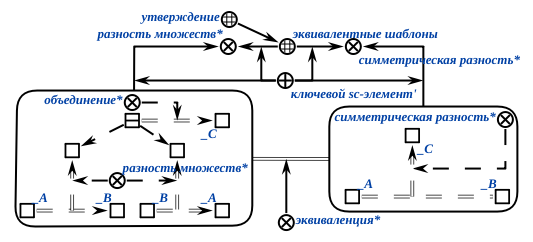
\includegraphics[scale=1]{author/part7/figures/equivalent_template_example.png}
		\caption{Пара шаблонов, удовлетворяющих логической эквивалентности}
		\label{fig:ET_example}
	\end{figure}
	
	\item использование двух шаблонов для поиска всех изоморфных семантических фрагментов в базе знаний и проверка наличия двух фрагментов пользователя в этих найденных фрагментах, которые соответственно включены в стандартный ответ и ответ пользователя. Если существуют такие два фрагмента (соответствие различным шаблонам), выполняется следующий шаг;
	
	\item итеративно проходятся разложенные подструктуры стандартного ответа и разложенные подструктуры ответа пользователя, и каждая подструктура сравнивается с соответствующим семантическим фрагментом, найденным на шаге 2, если каждый sc-элемент в подструктуре содержится в соответствующем семантическом фрагменте, подструктура удаляется;
	
	\item использование формул (\ref{formula_7_5_1}), (\ref{formula_7_5_2}) и (\ref{formula_7_5_3}) для вычисления подобия между семантическими фрагментами в соответствии с остальными подструктурами. Если подобие равно 1, то два семантических фрагмента полностью совпадают.
	
\end{enumerate}

Пример определения логической эквивалентности семантических фрагментов приведён на рисунке (\textit{\nameref{fig:LE_example}}) в \textit{SCg-коде}. 

Когда получено подобие ответов, можно проверить правильность и полноту ответов пользователей на объективные вопросы, объединив их со стратегией оценки объективных вопросов. Стратегия оценки объективных вопросов показана ниже:

\begin{textitemize}
	\item если для текущего тестового вопроса существует только один правильный вариант, только если стандартный ответ и ответ пользователя точно совпадают, ответ пользователя считается правильным, и пользователь получает максимальный балл ($Max_{score}$);
	
	\item если текущий вопрос имеет несколько правильных вариантов (например, вопросы на выбор с несколькими вариантами ответов и часть вопросов на заполнение пробелов):
	
	\begin{textitemize}
		\item до тех пор, пока ответ пользователя содержит неправильный вариант, ответ пользователя считается неправильным и оценка пользователя равна 0;
		
		\item если все варианты в ответе пользователя правильные, но количество правильных вариантов меньше, чем количество правильных вариантов в стандартном ответе, ответ пользователя считается правильным, но неполным. В это время оценка ответа пользователя равна $R_{sc}*Max_{score}$;
		
		\item если все варианты стандартного ответа точно совпадают со всеми вариантами ответа пользователя, то ответ пользователя точно правильный, а оценка пользователя равна $Max_{score}$. 	
		
	\end{textitemize}
	
\end{textitemize}

\begin{figure}[H]
	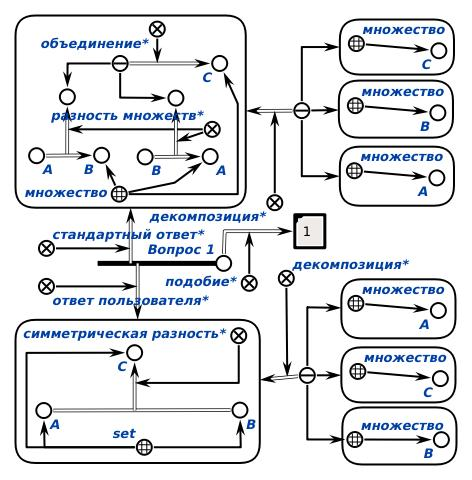
\includegraphics[scale=0.7]{author/part7/figures/logical_equivalence_example.jpg}
	\caption{Пример суждения логической эквивалентности семантических фрагментов, описанных на основе фактических знаний}
	\label{fig:LE_example}
\end{figure}

Пример проверки ответов на конкретный объективный вопрос показан на рисунке (\textit{\nameref{fig:AV_example}}) в \textit{SCg-коде}.

\subsubsection{Проверка ответов на субъективные вопросы}
\label{subsubsec_checking_answers_subjective_questions}

Наиболее важным этапом проверки ответов на субъективные вопросы также является вычисление подобия между семантическими фрагментами ответов, однако типы знаний и структуры знаний, используемые для описания различных типов субъективных вопросов и ответов на них, в \textit{ostis-системах} не одинаковы. Таким образом, подход к вычислению подобия между семантическими фрагментами ответов на субъективные вопросы далее делится на:

\begin{textitemize}
	\item подход к вычислению подобия между ответами на вопросы на толкование определений;
	\item подход к вычислению подобия между ответами на вопросы на доказательство и на решение задачи.
\end{textitemize} 
~\\
\textbf{Вычисление подобия между ответами на вопросы на толкование определений} 

~\\
Ответы на вопросы на толкование определений в \textit{ostis-системах} описываются в виде логических формул с использованием фактических знаний и логических знаний (\textit{Язык SCL}). Логическая формула является мощным инструментом для формального представления знаний в рамках \textit{Технологии OSTIS}, которая расширяется на основе формул логики предикатов первого порядка и наследует все операционные свойства формул логики предикатов первого порядка (см. \scncite{IMS}). Следует подчеркнуть, что при вычислении подобия между ответами на вопросы на толкование определений, фактические знания в семантических фрагментах ответов пользователей были согласованы с существующими знаниями в базе знаний (с использованием естественно-языковых интерфейсов) (см. \scncite{Qian2020}). Для вычисления подобия между семантическими фрагментами ответов на вопросы на толкование определений необходимо решить следующие задачи (см. \scncite{Fujiwara2021}):

\begin{textitemize}
	\item автоматический выбор потенциального эквивалентного стандартного ответа;
	\item установление отношений отображения потенциальных эквивалентных пар переменных sc-узлов между семантическими фрагментами ответов;
	\item вычисление подобия между семантическими фрагментами;
	\item если подобие между семантическими фрагментами не равно 1, то их также необходимо отдельно преобразовать в представление префиксной нормальной формы (п.н.ф./PNF), а затем снова вычислить подобие между ними.
\end{textitemize}

\begin{figure}[H]
	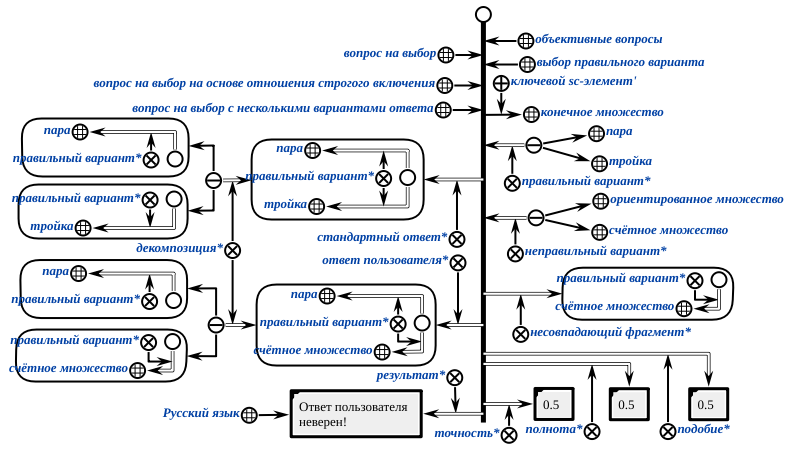
\includegraphics[scale=0.7]{author/part7/figures/answer_verification_example.png}
	\caption{Пример автоматической оценки вопроса на выбор с несколькими вариантами ответа}
	\label{fig:AV_example}
\end{figure}

Некоторые вопросы на толкование определений иногда имеют несколько стандартных ответов, но логические формулы, используемые для их формального представления, не являются логически эквивалентными (описываются в соответствии с различными системами понятий). Например, определение отношения эквивалентности:

\begin{textitemize}
	\item в математике отношение эквивалентности является бинарным отношением, которое является рефлексивным, симметричным и транзитивным;
	\item для любого бинарного отношения, если оно является толерантным отношением и транзитивным, то оно является отношением эквивалентности.
\end{textitemize}

Поэтому при вычислении подобия между ответами необходимо заранее отфильтровать стандартный ответ, который наилучшим образом соответствует ответу пользователя, из нескольких возможных стандартных ответов. Поэтому в данном параграфе предлагается подход к фильтрации стандартного ответа, который наилучшим образом соответствует ответу пользователя в соответствии с подобием предикатов между ответами. Принцип работы этого подхода показан ниже:

\begin{textitemize}
	\item нахождение всех предикатов в каждом ответе (неповторяющихся предикатов);
	\item вычисление подобия предикатов между ответом пользователя и каждым стандартным ответом с использованием формул (\ref{formula_7_5_1}), (\ref{formula_7_5_2}) и (\ref{formula_7_5_3}); 
	\item стандартный ответ, который наиболее похож (максимальное подобие) на ответ пользователя, выбирается в качестве окончательного стандартного ответа.
\end{textitemize}

Для того чтобы рассчитать подобие между семантическими фрагментами, наиболее важным шагом является установление отношений отображения потенциальных эквивалентных пар переменных sc-узлов между семантическими фрагментами. Поэтому на основе существующих методов отображения онтологий (например, ASMOW, RiMOM и др.) предлагается подход к установлению отношений отображения потенциальных эквивалентных пар переменных sc-узлов между семантическими фрагментами в соответствии с семантическими структурами (различными sc-конструкциями) (см. \scncite{Zeng2021, Sun2020, Rujiang2011}).

В \textit{ostis-системах} все \textit{логические связки} (такие как \textit{отрицание*} ($\lnot$) , \textit{импликация*} ($\to$) и так далее) и \textit{кванторами} (такие как \textit{квантор всеобщности} ($\forall$) и \textit{квантор существования} ($\exists$)) являются \textit{sc-связками} соответствующих отношений. Вопрос пользователя может быть представлен в виде атомарной логической формулы или \textit{конъюнкцией*} нескольких \textit{логических формул} (см. \scncite{Golenkov2014b, Rujiang2011}). Все sc-связки и sc-коннекторы образуют дерево, которое полностью описывает логическую последовательность между связками и кванторами в логической формуле. Поскольку sc-структура, содержащая атомарную логическую формулу, связана с соответствующим sc-связкой, пока определена позиция каждой sc-связки и sc-структуры в семантическом фрагменте, можно определить позицию каждой переменной sc-узла в этом семантическом фрагменте. В данном параграфе предлагается подход к нумерации каждой sc-связки и sc-структуры в семантическом фрагменте в соответствии со стратегией поиска в глубину (DFS). Процесс работы данного подхода показан ниже:

\begin{textitemize}
    \item каждая sc-связка и sc-структура в дереве нумеруется по очереди в соответствии со стратегией DFS и приоритетом текущей sc-связки (например, приоритет sc-связки ``если' ''\ выше, чем приоритет sc-структуры ``то' '') (последовательность нумерации начинается с 0);
	\item в соответствии с последовательностью нумерации sc-связок, каждый sc-связка в дереве обходится от малого к большому, а sc-структура, связанная с текущей sc-связкой, нумеруется при обходе (последовательность нумерации начинается с 1).
\end{textitemize}

При проверке ответа, если стандартный ответ и ответ пользователя точно равны, это означает, что атомарные логические формулы с одинаковой семантикой между ответами имеют одинаковое положение в семантическом фрагменте (то есть, последовательность нумерации sc-структуры одинакова). Поэтому в данном параграфе отношения отображения потенциальных эквивалентных пар переменных sc-узлов будут устанавливаться на основе отношений соответствия sc-конструкций в одной и той же позиции между ответами. Процесс установления отношений отображения потенциальных эквивалентных пар переменных sc-узлов между ответами показан ниже:

\begin{enumerate}
	\item в соответствии с последовательностью нумерации sc-структур в семантическом фрагменте, каждый раз, когда из стандартного ответа и ответа пользователя найдена пара sc-структур с одинаковым номером;
	\item в соответствии с порядком приоритета (от высокого к низкому) различных типов sc-конструкций, используемых для описания атомарной логической формулы, поочередно определяется, содержит ли текущая пара sc-структур одновременно данный тип sc-конструкции. Если этот тип sc-конструкции одновременно содержится в текущей паре sc-структур, то, в соответствии с отношением соответствия каждого sc-элемента между текущей sc-конструкцией в стандартном ответе и текущей sc-конструкцией в ответе пользователя, устанавливаются отношения отображения потенциальных эквивалентных пар переменных sc-узлов между текущими sc-конструкциями;
	\item повторять шаг 1 --- шаг 2, пока не будут установлены все отношения отображения между семантическими фрагментами (см. \scncite{Li2021}).
\end{enumerate}

На рисунке (\textit{\nameref{fig:EMR_example}}) рассмотрено установление отношений отображения между семантическими фрагментами в \textit{SCg-коде}.

Когда отношения отображения потенциальных эквивалентных пар переменных sc-узлов между семантическими фрагментами установлены, можно вычислить подобие между ответами. Ниже показан процесс вычисления подобия между семантическими фрагментами ответов на вопросы на толкование определений:

\begin{textitemize}
	\item декомпозиция семантического фрагмента стандартного ответа и семантического фрагмента ответа пользователя на подструктуры в соответствии с правилами представления фактических знаний и логических знаний;
	\item нумерация sc-связок и sc-структур в семантических фрагментах ответов, соответственно, и установление отношений отображения потенциальных эквивалентных пар переменных sc-узлов между семантическими фрагментами;
	\item использование формул (\ref{formula_7_5_1}), (\ref{formula_7_5_2}) и (\ref{formula_7_5_3}) для вычисления точности $P_{sc}$, полноты $R_{sc}$ и подобия $F_{sc}$ между семантическими фрагментами. 
\end{textitemize}

Поскольку семантические фрагменты ответов на вопросы на толкование определений описываются на основе логических формул, если подобие между семантическими фрагментами не равно 1 ($F_{sc}$ < 1), необходимо также определить, являются ли их логические формулы логически эквивалентными. В логике предикатов существует такая теорема: любая формула логики предикатов имеет эквивалентную ей \textit{п.н.ф.} Поскольку логическая формула в рамках \textit{Технологии OSTIS} расширяется на основе формулы логики предикатов, она также обладает таким свойством. Поэтому мы можем рассмотреть возможность преобразования семантических фрагментов, основанных на описаниях логических формул, в описания \textit{п.н.ф.}, а затем определить, удовлетворяется ли между ними логическая эквивалентность (см. \scncite{Fujiwara2021, Kowalski1974}). Однако \textit{п.н.ф.} логической формулы не является уникальной, и причины, по которым п.н.ф. не является уникальной, включают:

\begin{textitemize}
	\item используемый порядок различных формул логической эквивалентности (правила преобразования). Например, преобразование ($\forall x F(x) \land \neg \exists x G(x)$) в \textit{п.н.ф.}:
	
	\begin{textitemize}
		\item $\forall x F(x) \land \neg \exists x G(x)$ \\ $\Leftrightarrow$ $\forall x F(x) \land \forall x \neg G(x)$ \\ $\Leftrightarrow$ $\forall x (F(x) \land \neg G(x)) $, (правило эквивалентности) 
		\item $\forall x F(x) \land \neg \exists x G(x)$ \\ $\Leftrightarrow$ $\forall x F(x) \land  \forall y \neg G(y)$, (правила переименования) \\ $\Leftrightarrow$ $\forall x \forall y (F(x) \land \neg G(y)) $, (правила расширения области действия кванторов)
	\end{textitemize}
	
	\item порядок кванторов в \textit{п.н.ф.} Например, преобразование логической формулы ($\forall x F(x)\wedge \exists y G(y)$) в \textit{п.н.ф.}:
	
	\begin{textitemize}
		\item $\forall x F(x)\wedge \exists y G(y)$ \\
		$\Leftrightarrow$ $\forall x \exists y (F(x) \wedge G(y))$, (правила расширения области действия кванторов)
		\item $\forall x F(x)\wedge \exists y G(y)$ \\
		$\Leftrightarrow$ $\exists y \forall x (F(x) \wedge G(y))$, (правила расширения области действия кванторов)
	\end{textitemize}
	
\end{textitemize}

\begin{figure}[H]
	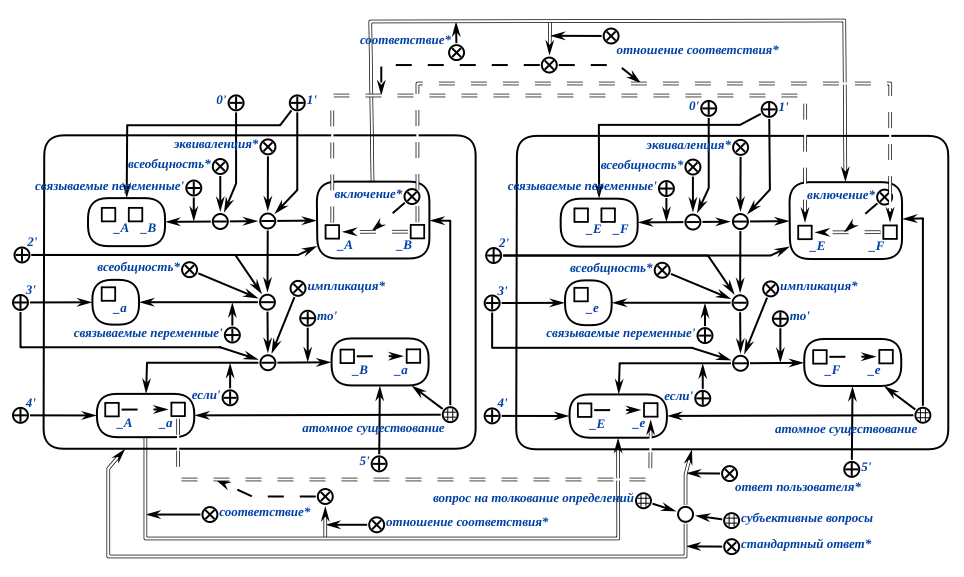
\includegraphics[scale=0.65]{author/part7/figures/establishment_mapping_relationship_example.png}
	\caption{Пример установления отношений отображения потенциальных эквивалентных пар переменных sc-узлов между семантическими фрагментами}
	\label{fig:EMR_example}
\end{figure}

Поэтому, на основе подхода к преобразованию формул логики предикатов в \textit{п.н.ф.} и некоторых характеристик логических формул в \textit{ostis-системах}, в данном параграфе предлагается подход к преобразованию логических формул в уникальные (детерминированные) \textit{п.н.ф.} в соответствии со строгими правилами ограничения. Строгие правила ограничения в основном включают следующее:

\begin{textitemize}
	\item чтобы решить проблему, заключающуюся в том, что \textit{п.н.ф.} не являются уникальными из-за порядка использования различных формул логической эквивалентности, мы указываем, что правило переименования должно использоваться предпочтительно при преобразовании логических формул в \textit{п.н.ф.};
	
	\item для решения проблемы, что \textit{п.н.ф.} не является уникальной из-за порядка кванторов, в данном параграфе предлагается подход, позволяющий перемещать все кванторы в передний конец логической формулы строго в соответствии с приоритетом кванторов. Процесс перемещения кванторов показан ниже:
	
	\begin{textitemize}
		\item если в начале логической формулы не существует кванторов, то все кванторы существования перемещаются в начало логической формулы по преимуществу;
		
		\item если последний квантор в переднем конце логической формулы является квантором всеобщности, то кванторы всеобщности в логической формуле будут преимущественно перемещены в начало формулы;
		
		\item если последний квантор в переднем конце логической формулы является квантором существования, то кванторы существования в логической формуле будут перемещены преимущественно в начало формулы.
	\end{textitemize}
	
	\item логическая формула, используемая для представления ответа на вопрос на толкование определений, обычно может быть выражена в следующей форме: ($Q_{1}x_{1}Q_{2}x_{2}\cdots Q_{n}x_{n}(A\leftrightarrow B)$), где $Q_{i}\left ( i = 1, \cdots n \right )$ представляет собой квантор (см. \scncite{Li2021, Krom1970}). $A$ используется для описания определения понятия на целостном уровне, и кванторы в него не включены. $B$ используется для объяснения семантического оттенка определения на уровне детализации, и обычно эта формула является логической формулой, содержащей кванторы (также известной как логическая подформула). Поэтому, исходя из характеристик логической формулы и для упрощения обработки знаний, необходимо лишь преобразовать логическую формулу $B$ в \textit{п.н.ф.};
	
	\item для упрощения обработки знаний при преобразовании логических формул в \textit{п.н.ф.} необходимо исключить только связку импликации;
	
	\item несколько атомарных логических формул, соединённых с помощью одной и той же связки конъюнкции, предпочтительно объединяются в одно целое (то есть они объединяются в одну sc-структуру).
	
\end{textitemize}

Процесс преобразования семантических фрагментов ответов на вопросы на толкование определений в описание п.н.ф. в соответствии со строгими правилами ограничения показан ниже:

\begin{textitemize}
	\item если в семантическом фрагменте имеется несколько sc-структур, соединённых одной и той же связкой конъюнкции, то содержащиеся в них sc-конструкции объединяются в одну sc-структуру;
	
	\item исключение всех связок импликации в семантических фрагментах;
	
	\item перемещение всех связок отрицания в семантических фрагментах в передний конец соответствующей sc-структуры;
	
	\item использование правила переименования, чтобы все связанные переменные в семантических фрагментах не были одинаковыми;
	
	\item перемещение всех кванторов в первый конец логической формулы;
	
	\item снова объединение sc-структур, которые могут быть объединены в семантическом фрагменте.
	
\end{textitemize}

Пример преобразования логической формулы в \textit{п.н.ф.} показан на рисунке (\textit{\nameref{fig:PNF_example}}) в \textit{SCg-коде} ($\forall A\forall B((A\subseteq B) \leftrightarrow \forall a(a\in A\rightarrow a\in B))$ $\Leftrightarrow$ $\forall A\forall B((A\subseteq B) \leftrightarrow \forall a ( \neg ( a\in A ) \lor (a\in B)))$).

\begin{figure}[H]
	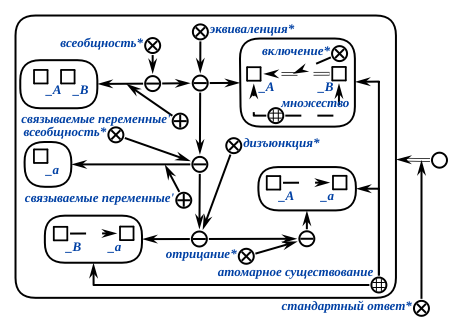
\includegraphics[scale=0.8]{author/part7/figures/PNF_example.png}
	\caption{Пример преобразования семантического фрагмента в представление п.н.ф.}
	\label{fig:PNF_example}
\end{figure}

Следует подчеркнуть, что если вычисленное подобие между семантическими фрагментами представления \textit{п.н.ф.} не равно 1 ($F_{sc}$ < 1), то в качестве окончательного подобия ответа используется подобие между семантическими фрагментами, вычисленное в первый раз. Когда подобие между ответами получено, а затем объединено со стратегией оценки субъективных вопросов, можно проверить правильность и полноту ответов пользователей (см. \scncite{Li2021}).

~\\
\textbf{Вычисление подобия между ответами на вопросы на доказательство и на решение задачи} 

~\\
Как вопросы на доказательство, так и решение задачи в математике следуют общему процессу решения задач:

\begin{enumerate}
	\item набор условий ($\Omega $), состоящий из некоторых известных условий;
	
	\item выведение промежуточного вывода с использованием некоторых известных условий в $\Omega $ и добавление его к $\Omega $. Каждый элемент в $\Omega $ можно рассматривать как шаг решения;
	
	\item повторять шаг 2 до получения окончательного результата (см. \scncite{Zhang1995, Zhang2019}).
\end{enumerate}

Этот процесс решения задачи абстрагируется в виде направленного графа, структура которого в большинстве случаев представляет собой перевернутое дерево (в особых случаях направленный граф будет содержать цикл), (рисунок \textit{\nameref{fig:RT_example}}), и называется деревом рассуждений (то есть деревом рассуждений стандартного ответа).

\begin{figure}[H]
	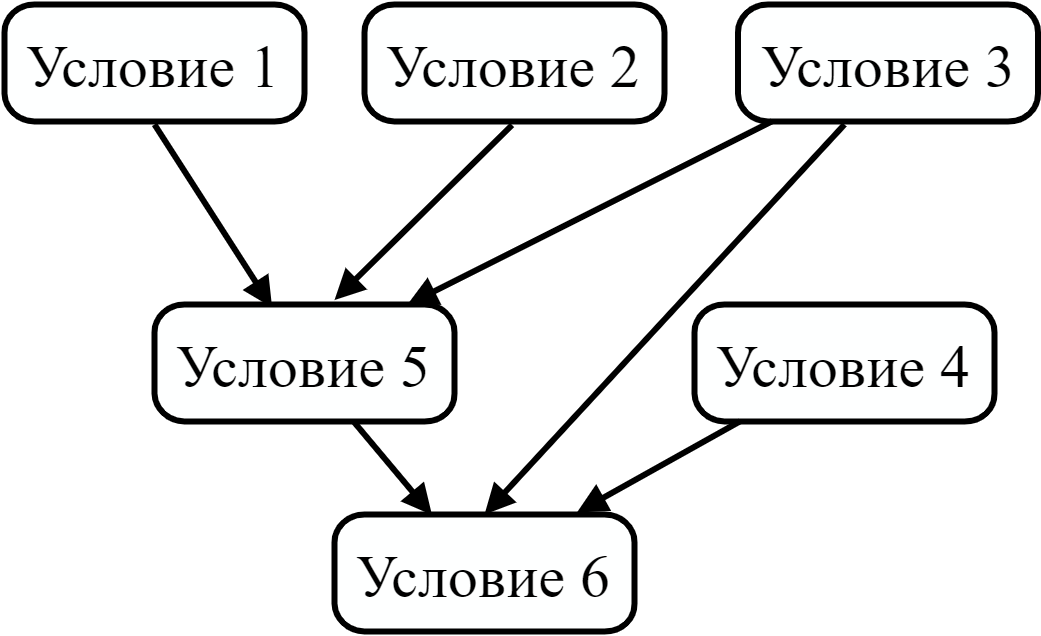
\includegraphics[scale=0.15]{author/part7/figures/reasoning_tree_example.png}
	\caption{Пример дерева рассуждений}
	\label{fig:RT_example}
\end{figure}

Ответ пользователя на вопрос на доказательство или на решение задачи представляет собой линейную структуру, состоящую из некоторых шагов решения (то есть известных условий, промежуточных условий или выводов), каждый из которых удовлетворяет строгим отношениям выведения и логическим отношениям, если ответ пользователя полностью правильный. Процесс автоматической проверки ответов пользователя на данный тип тестовых вопросов аналогичен традиционной ручной проверке ответов, то есть проверка того, является ли текущий шаг решения ответа пользователя правильным заключением частичного шага решения, предшествующего этому шагу. Это означает, всегда ли шаг решения в ответе пользователя, соответствующий родительскому узлу в дереве рассуждений, располагается после шагов решения в ответе пользователя, соответствующих дочерним узлам.

Семантические фрагменты ответов пользователя на вопросы на доказательство и на решение задачи в \textit{ostis-системах} представляют собой линейные структуры, состоящие из некоторых семантических подфрагментов для описания шагов решения и некоторых семантических фрагментов для описания логического порядка и процессов преобразования между семантическими подфрагментами (см. \scncite{Golenkov2014b, IMS}). Процесс построения и семантическая спецификация семантических фрагментов ответов пользователя на вопросы на доказательство и на решение задачи подробно описаны в работе (см. \scncite{Shunkevich2015}). Семантические фрагменты стандартных ответов на тестовые вопросы такого типа представляют собой деревья рассуждений, состоящие из некоторых шаблонов поиска (которые могут абстрагироваться как узлы в дереве). Каждый шаблон поиска построен строго в соответствии со стандартными шагами решения соответствующего тестового вопроса (то есть в соответствии с известными условиями, промежуточными условиями и выводами в $\Omega $). Шаблон поиска в \textit{ostis-системах} используется для поиска в базе знаний всех соответствующих ему семантических фрагментов, и он построен на основе \textit{Языка SCL}. Далее в качестве примера взято реальное решение задачи, чтобы представить построение его семантического фрагмента ответа пользователя (рисунок \textit{\nameref{fig:STE_example}}) и семантического фрагмента стандартного ответа (дерева рассуждений), (рисунок \textit{\nameref{fig:ITE_example}}). Описание решения задачи: <<Две равные окружности внешне касаются другой и третьей окружности, радиус которой равен 4. Отрезок, торой соединяет точки касания двух равных окружностей с третьей, равен 6. Найдите радиусы равных окружностей.>>, (рисунок \textit{\nameref{fig:EI_example}}).

\begin{figure}[H]
	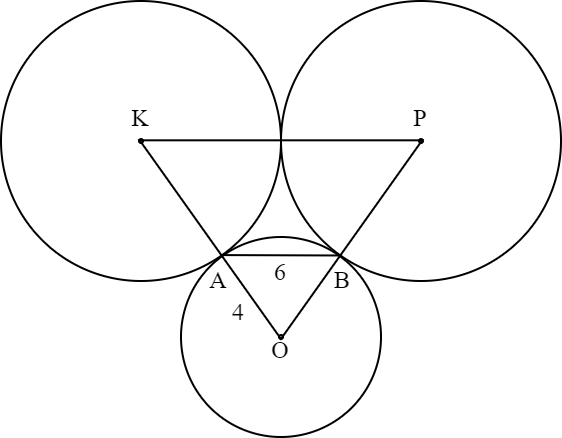
\includegraphics[scale=0.3]{author/part7/figures/explanatory_illustration_example.png}
	\caption{Пояснительный рисунок к решению задачи}
	\label{fig:EI_example}
\end{figure}

Описание ответа пользователя на естественном языке:

\begin{enumerate}
	\item $\because KP = 2*R$
	\item $\because KO = 4+R$
	\item $\therefore \Delta A O B\backsim \Delta K O P$
	\item $\therefore K A = R = 12$
\end{enumerate}

Ответы пользователей на естественном языке преобразуются в семантические фрагменты с помощью естественно-языковых интерфейсов. Поэтому при вычислении подобия между семантическими фрагментами ответов нет необходимости учитывать различия понятий на уровне \textit{естественного языка} (см. \scncite{Qian2020}). Пример спецификации конкретного понятия показан на рисунке (\textit{\nameref{fig:SSE_example}}).

\begin{figure}[H]
	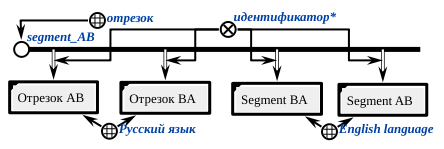
\includegraphics[scale=0.8]{author/part7/figures/specification_segment_example.png}
	\caption{Пример семантической спецификации отрезка AB}
	\label{fig:SSE_example}
\end{figure}

\begin{figure}[H]
	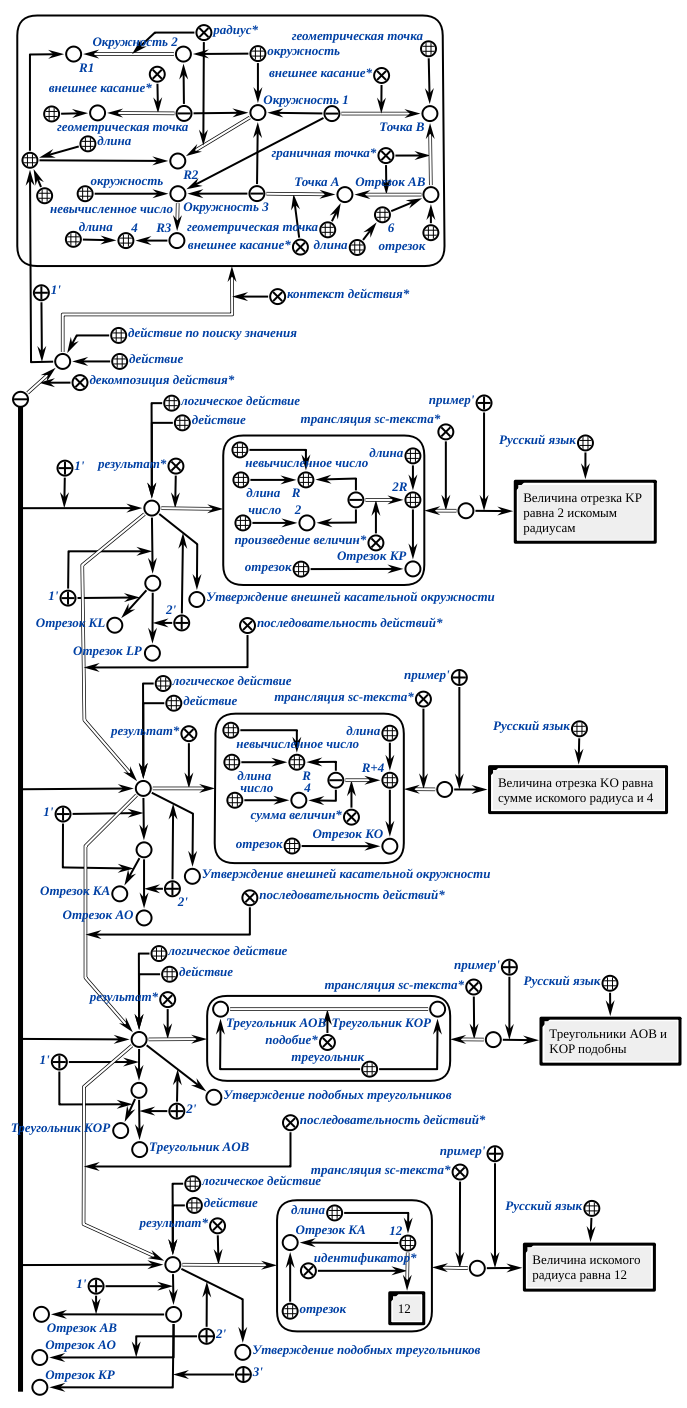
\includegraphics[scale=0.7]{author/part7/figures/solving_task_example.png}
	\caption{Пример семантической модели ответа пользователя на решение задачи}
	\label{fig:STE_example}
\end{figure}

\begin{figure}[H]
	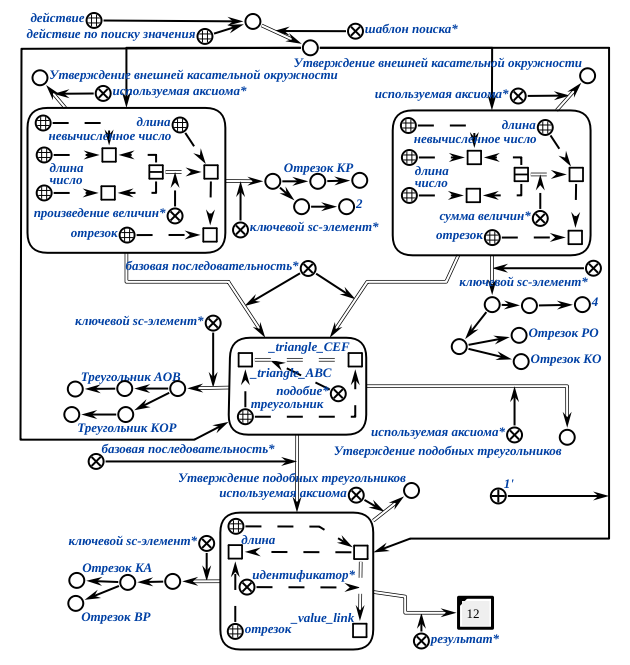
\includegraphics[scale=0.6]{author/part7/figures/inference_tree_example_SCg.png}
	\caption{Пример семантической модели дерева рассуждений стандартного ответа}
	\label{fig:ITE_example}
\end{figure}

Из рисунка (\textit{\nameref{fig:SSE_example}}) видно, что \textit{Отрезок AB} и \textit{Отрезок BA} представлены одним и тем же sc-узлом, они просто являются двумя идентификаторами sc-узла. Поэтому на основе ранее представленного принципа автоматической проверки ответов пользователя на вопросы на доказательство и на решение задачи и семантических моделей ответов в \textit{ostis-системах}, в данном параграфе предлагается подход к вычислению подобия между семантическими фрагментами ответов на вопросы на доказательство и на решение задачи в соответствии с деревом рассуждений стандартного ответа (семантический фрагмент стандартного ответа). Процесс вычисления подобия между семантическими фрагментами показан ниже:

\begin{enumerate}
	\item нумерация каждого семантического подфрагмента (шага решения) в семантическом фрагменте ответов пользователей (порядок нумерации начинается с 1);
	
	\item каждый узел (шаблон поиска) в дереве рассуждений обходится по очереди в соответствии со стратегией DFS. В то же время, соответствующий семантический подфрагмент, включенный в семантический фрагмент ответа пользователя, ищется в базе знаний с использованием шаблона поиска, который обходится в данный момент. Если такой семантический подфрагмент существует, то определить, меньше ли нумерация найденного семантического подфрагмента, чем нумерация семантического подфрагмента, соответствующего шаблону поиска родительского узла текущего шаблона поиска (кроме корневого узла дерева рассуждений), и если да, то найденный семантический подфрагмент считается правильным;
	
	\item повторять шаг 2, пока не будут обойдены все шаблоны поиска в дереве рассуждений и одновременно подсчитано количество правильных семантических подфрагментов;
	
	\item использование формул (\ref{formula_7_5_1}), (\ref{formula_7_5_2}) и (\ref{formula_7_5_3}) для вычисления точности $P_{sc}$, полноты $R_{sc}$ и подобия $F_{sc}$ между ответами. Параметры в формуле переопределены:
	
	\begin{textitemize}
		\item $|T_s{_c}(u)|$ --- количество всех семантических подфрагментов в семантическом фрагменте ответа пользователя $u$; 
		\item $|T_s{_c}(s)|$ --- количество всех шаблонов поиска в дереве рассуждений $s$; 
		\item $|T_s{_c}(u)\otimes T_s{_c}(s)|$ --- количество правильных семантических подфрагментов.
	\end{textitemize}
	
\end{enumerate}

После получения подобия между ответами на вопросы на доказательство и на решение задачи, правильность и полнота ответов пользователей может быть проверена в сочетании со стратегией оценки субъективных вопросов.

Стратегия оценки субъективных вопросов показана ниже:

\begin{textitemize}
	\item если подобие между ответами равно 1 ($F_{sc}$ = 1), то ответ пользователя полностью правильный и пользователь получает максимальный балл ($Max_{score}$);
	
	\item если подобие между ответами меньше 1 ($F_{sc}$ < 1) и точность равна 1 ($P_{sc}$ = 1), то ответ пользователя правильный, но неполный, и оценка пользователя равна $R_{sc}*Max_{score}$;
	
	\item если подобие между ответами больше 0 и меньше 1, а точность меньше 1 (0 < $F_{sc}$ < 1 и $P_{sc}$ < 1), то ответ пользователя является частично правильным и оценка пользователя равна $P_{sc}*Max_{score}$;
	
	\item если подобие между ответами равно 0 ($F_{sc}$ = 0), то ответ пользователя является неправильным и оценка пользователя равна 0 (см. \scncite{Li2021}).
\end{textitemize}

Предлагаемый подход к автоматической проверке ответов пользователей имеет следующие преимущества:

\begin{textitemize}
	\item проверка правильности и полноты ответов пользователя на основе семантики;
	
	\item можно проверить правильность и полноту ответов пользователя на любые типы тестовых вопросов и определить логическую эквивалентность между ответами;
	
	\item позволяет вычислять подобие между любыми двумя семантическими фрагментами в базе знаний;
	
	\item предложенный подход может быть использован в различных \textit{ostis-системах}.
\end{textitemize}

\subsection{Семантическая модель базы знаний подсистемы контроля знаний}
\label{subsec_semantic_model_KB_knowledge_control_subsystem}

База знаний подсистемы в основном используется для хранения автоматически сгенерированных тестовых вопросов различных типов, а также позволяет автоматически извлекать ряд тестовых вопросов и формировать экзаменационные билеты в соответствии с требованиями пользователя. Поэтому для повышения эффективности доступа к базе знаний подсистемы и эффективности извлечения тестовых вопросов в данном параграфе предлагается подход к построению базы знаний подсистемы в соответствии с типом тестовых вопросов и стратегией генерации тестовых вопросов. Основой базы знаний любой \textit{ostis-системы} (точнее, sc-моделью \textit{базы знаний}) является иерархическая система предметных областей и соответствующих им онтологий (см. \scncite{Golenkov2014b, Shunkevich2015, IMS}). Рассмотрим иерархию базы знаний подсистемы в \textit{SCn-коде}:
\begin{SCn}
	\scnheader{Раздел. Предметная область тестовых вопросов}
	
	\begin{scnreltoset}{декомпозиция раздела}
		
		\scnitem{Раздел. Предметная область субъективных вопросов}
		
		\begin{scnreltoset}{декомпозиция раздела}
			\scnitem{Раздел. Предметная область вопроса на толкование определений}
			\scnitem{Раздел. Предметная область вопроса на доказательство}
			\scnitem{Раздел. Предметная область решения задачи}
		\end{scnreltoset}
		
		\scnitem{Раздел. Предметная область объективных вопросов}
		
		\begin{scnreltoset}{декомпозиция раздела}
			\scnitem{Раздел. Предметная область вопроса на выбор}
			\scnitem{Раздел. Предметная область вопроса на заполнение пробелов}
			\scnitem{Раздел. Предметная область вопроса суждения}
		\end{scnreltoset}
		
	\end{scnreltoset}
\end{SCn}

Далее, взяв в качестве примера предметную область объектных вопросов, рассмотрим ее структурную спецификацию в \textit{SCn-коде}:
\begin{SCn}
	\scnheader{Предметная область объективных вопросов}
	\scniselement{предметная область}
	\scnhaselementrole{максимальный класс объектов исследования}{объективный вопрос}
	\begin{scnhaselementrolelist}{немаксимальный класс объектов исследования}
		\scnitem{вопрос на выбор}
		\scnitem{вопрос на заполнение пробелов}
		\scnitem{вопрос суждения} 
	\end{scnhaselementrolelist}
\end{SCn}

Объективные типы тестовых вопросов могут быть разложены на более конкретные типы в соответствии с их характеристиками и соответствующими стратегиями генерации тестовых вопросов. Далее, взяв в качестве примера вопрос на выбор, рассмотрим его семантическую спецификацию в \textit{SCn-коде}:

\begin{SCn}
	\scnheader{вопрос на выбор}
	\scniselementrole{максимальный класс объектов исследования}{Предметная область вопроса на выбор}
	
	\begin{scnrelfromset}{разбиение}
		
		\scnitem{вопрос на выбор на основе свойств отношений}
		\scnitem{вопрос на выбор на основе идентификаторов}
		\scnitem{вопрос на выбор на основе примеров изображения}
		\scnitem{вопрос на выбор на основе аксиом}
		\scnitem{вопрос на выбор на основе элементов}
		
		\begin{scnrelfromset}{разбиение}
			\scnitem{вопрос на выбор на основе бинарного отношения}
			\scnitem{вопрос на выбор на основе ролевого отношения}
		\end{scnrelfromset}
		
		\scnitem{вопрос на выбор на основе классов}
		
		\begin{scnrelfromset}{разбиение}
			\scnitem{вопрос на выбор на основе отношения разбиения}
			\scnitem{вопрос на выбор на основе отношения строгого включения}
			\scnitem{вопрос на выбор на основе отношения включения}
		\end{scnrelfromset}
		
	\end{scnrelfromset}
	
	\begin{scnrelfromset}{разбиение}
		\scnitem{вопрос на выбор с несколькими вариантами ответа}
		\scnitem{вопрос на выбор с одним вариантом ответа}
	\end{scnrelfromset}
	
	\begin{scnrelfromset}{разбиение}
		\scnitem{выбор неправильного варианта}
		\scnitem{выбор правильного варианта}
	\end{scnrelfromset}
\end{SCn}

\subsection{Семантическая модель решателя задач подсистемы контроля знаний}
\label{subsec_semantic_model_problem_solver_knowledge_control_subsystem}

Решатель задач любой \textit{ostis-системы} (точнее, sc-модель решателя задач \textit{ostis-системы}) представляет собой иерархическую систему sc-агентов обработки знаний в семантической памяти (sc-агенты), которые взаимодействуют только путем указания действий, выполняемых ими в указанной памяти (см. \scncite{Golenkov2014b}).

Поэтому для решения соответствующих задач в данном параграфе приведена реализация решателя задач для автоматической генерации тестовых вопросов и автоматической проверки ответов пользователей, иерархия которого представлена следующим образом в \textit{SCn-коде}:

\begin{SCn}
	\scnheader{Решатель задач для автоматической генерации тестовых вопросов и автоматической проверки ответов пользователей}
	
	\begin{scnrelfromset}{декомпозиция абстрактного sc-агента}
		
		\scnitem{Абстрактный sc-агент для автоматической генерации тестовых вопросов}
		
		\begin{scnrelfromset}{декомпозиция абстрактного sc-агента}
			\scnitem{Абстрактный sc-агент для быстрой генерации тестовых вопросов и экзаменационных билетов}
			\scnitem{Абстрактный sc-агент для генерации тестовых вопросов одного типа}
			\scnitem{Абстрактный sc-агент для генерации единого экзаменационного билета}
		\end{scnrelfromset}
		
		\scnitem{Абстрактный sc-агент для автоматической проверки ответов пользователей}
		
		\begin{scnrelfromset}{декомпозиция абстрактного sc-агента}
			\scnitem{Абстрактный sc-агент для автоматической оценки экзаменационных билетов}
			\scnitem{Абстрактный sc-агент для вычисления подобия между ответами на объективные вопросы}
			\scnitem{Абстрактный sc-агент для оценки логической эквивалентности между семантическими фрагментами, описанными на основе фактических знаний}
			\scnitem{Абстрактный sc-агент для вычисления подобия между ответами на вопросы на толкование определений}
			\scnitem{Абстрактный sc-агент для преобразования логической формулы в п.н.ф.}
			\scnitem{Абстрактный sc-агент для вычисления подобия между ответами на решение задачи и на вопросы на доказательство}
		\end{scnrelfromset}
		
	\end{scnrelfromset}
\end{SCn}

Основная функция абстрактного \textit{sc-агента} для быстрой генерации тестовых вопросов и экзаменационных билетов заключается в автоматизации всего процесса от генерации тестовых вопросов до генерации экзаменационных билетов путём инициирования соответствующих \textit{sc-агентов} (абстрактный \textit{sc-агент} для генерации тестовых вопросов одного типа и абстрактный sc-агент для генерации единого экзаменационного билета). Основной функцией абстрактного sc-агента для генерации тестовых вопросов одного типа является автоматическая генерация ряда тестовых вопросов из базы знаний с использованием логических правил, построенных на основе \textit{SC-кода} (см. \scncite{IMS}). Логические правила для генерации тестовых вопросов построены строго в соответствии со стратегиями генерации тестовых вопросов, описанными ранее. Пример логического правила приведён на рисунке (\textit{\nameref{fig:LRE_example}}).

\begin{figure}[H]
	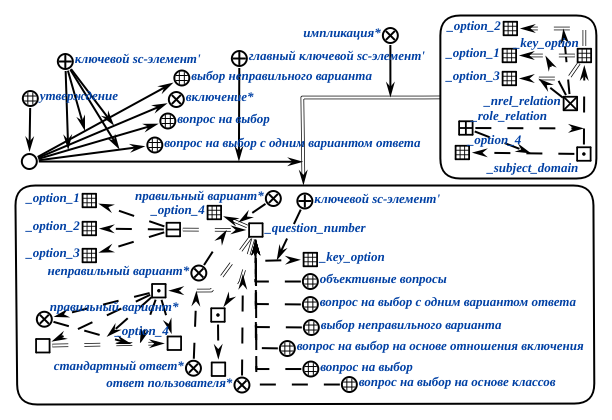
\includegraphics[scale=1]{author/part7/figures/logic_rule_example.png}
	\caption{Пример логического правила для генерации вопроса на выбор}
	\label{fig:LRE_example}
\end{figure}

Основная функция абстрактного \textit{sc-агента} для автоматической оценки экзаменационных билетов заключается в реализации автоматической проверки ответов пользователей на различные типы тестовых вопросов и автоматической оценки экзаменационных билетов путём инициирования абстрактных \textit{sc-агентов} для вычисления подобия между ответами пользователей, абстрактного \textit{sc-агента} для оценки логической эквивалентности между семантическими фрагментами, описанными на основе фактических знаний и абстрактного \textit{sc-агента} для преобразования логической формулы в \textit{п.н.ф.}